\section{First day of operations}\label{first-day-of-operations}
We have commenced the first image acquisition in the light microscopy module (LMM) as part of the ACE-M2 experiment. The LMM system is being controlled directly by the Payload Developer (PD), Lou Chesney, sitting at the bank of computer screens that run the control software:
\begin{figure}[h]
\begin{center}
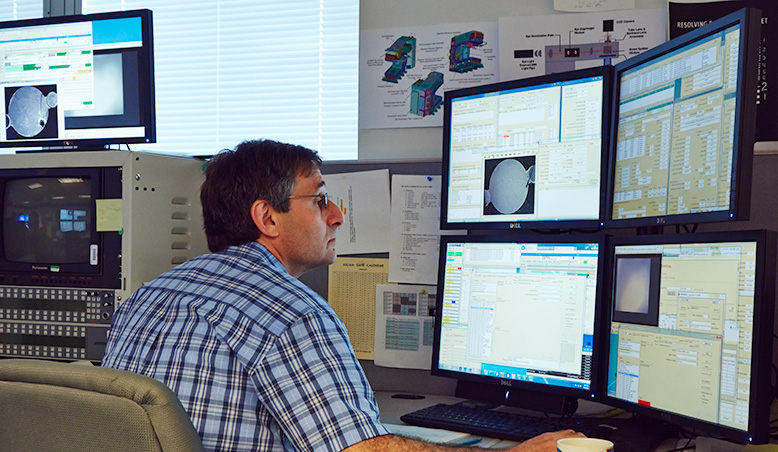
\includegraphics[width=3.1in]{./images/2014_06_04_first_day/140604_ace_tsc_chestney_lou_web.jpg}
\end{center}
\caption{Lou Chesney}
\end{figure}

Because the microscope is onboard the International Space Station, the communications between the commands Lou issues on the ground, and what happens on orbit depends on close coordination with the general communications with the ISS. In particular, there are frequent interruptions of communications and controls, depending on where in its flight path the Space Station is, relative to the geostationery satellites that relay its communications first to Marshall Space Flight Center (MSFC) in Huntsville, Alabama, then to the Telescience Center (TSC) here at NASA Glenn Research Center (GRC) here in Cleveland. The rack officer (RO) coordinates these communications, and integrates the specific timing of operations with the general ISS timeline; this morning, Jim Birchenough is serving in both this role, and as the data management officer (DMO)---overseeing the data downlink so we can live previews and downloaded images---and has his own bank of screens to monitor:
\begin{figure}[h]
\begin{center}
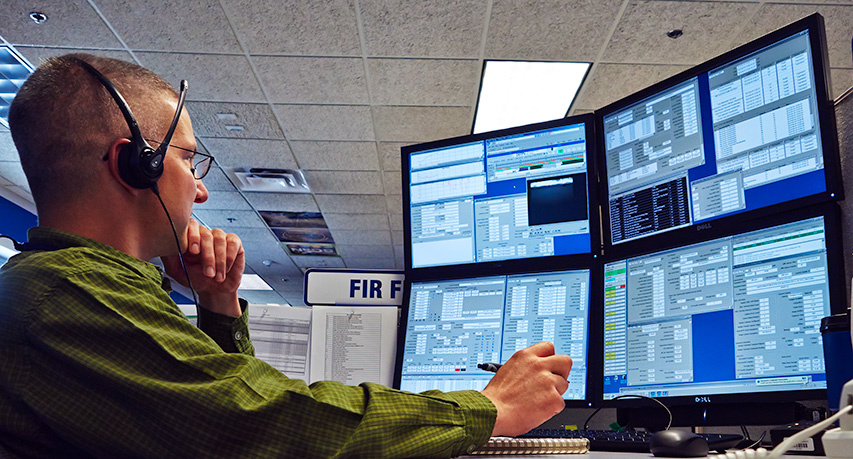
\includegraphics[width=\columnwidth]{./images/2014_06_04_first_day/140604_ace_tsc_birchenough_james_web.jpg}
\end{center}
\caption{James Birchenough}
\end{figure}

After a full 8-hour shift, Lou and James swapped positions with Tibor Lorik (PD) and Amber Krauss (RO / DMO):
\begin{figure}[h]
\begin{center}
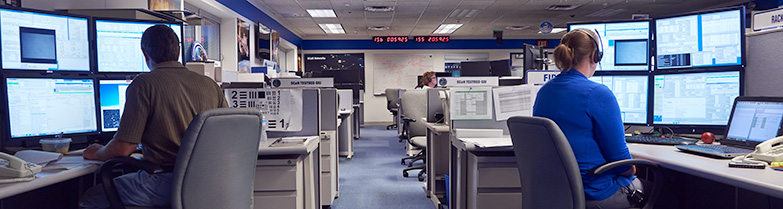
\includegraphics[width=\columnwidth]{./images/2014_06_04_first_day/140604_ace_tsc_tibor_amber_web.jpg}
\end{center}
\caption{Tibor Lorik and Amber Krauss}

\end{figure}

